
    XXX muss vmtl eig in BAsics
    To evaluate the quality of the material parameters we need a possibility to investigate the material response caused by the definition of the material parameters. Then we can compare this results with the load parameters and evaluate the quality of the current material parameters. Thus we have to use a simulation program to analyse the material behaviour for every iteration of material parameter values during the optimisation process. We decided to use \name{abaqus} as simulation software, because of the intern scripting tool. With the \name{abaqus} scripting tool one can run python scripts directly in \name{abaqus} (see chapter XX). With special \name{abaqus} commands one can use \name{abaqus} with the same opportunities as with the GUI. 
    XXXX

    Therefore we choose simple load cases, which are easy to recalculate. AS explained in the chpater XX about the mathematical problem formulation, we have to define a parameter which defines the quality of the mechanical responses calculated by \name{abaqus} compared to the ones from the MD-simulation. Therefore we first have to define adequate mechanical measurements which represent best the mechanical behaviour and contain information about the material parameters. Hence the stress and strain measurements in all normal and shear directions are possible quantities. Depending on the load case the measurements with the most useful information may vary.
    

    
    \chapter{Models and Methods}

    In the following chapter we describe the optimisation process used in this thesis. Therefore we first have a closer look on the theoretical structure of the process. Afterwards we introduce the necessary input data. Then the structure of the code is presented. 

    \section{Theory} \label{sec: methodTheory}

    The aim of the optimisation process is to find material parameters which best represent the mechanical behaviour analysed with a MD-Simulation. In the following we demonstrate the need of this process.
    The MD-analysis gives information about the mechanical response for an applied load case. In a MD-simulation we can apply a load case and log the stress and strain values in all directions at prescribed time steps during the loading process. In the following this data from the MD-Simulations are called load parameters. They describe the applied load (for example uniform strain up to 20\(\%\)) and the corresponding reactions. In \autoref{subsec:loadParameters} we have a closer look on the structure of the data. 
    This load parameters empirically describe the mechanical behaviour of the investigated material. However, we are interested in a deterministic description of the material behaviour. This is usually done by the definition of material parameters. Since it is not possible to specify material parameters directly in the MD-simulation, we want to build a optimisation process which is able to find the best material parameters to represent the material behaviour from the load parameters. To implement this problem we have to reformulate it as a minimization problem. As minimization value we have to define a value that represents the error of mechanical response of the material. Therefore we compare the material behaviour defined through the material parameters with the one from the load parameters. If we minimize their difference, we improve the quality of the material parameter values describing the material behaviour. In our problem formulation we have now the optimisation of the material parameters controlled by the minimization of the difference between the mechanical responses. In the next step we need to define this difference between the mechanical behaviour more precisely. For the mathematical formulation only one single value is allowed for the problem formulation. For a detailed explanation we now introduce the used model, the load cases and load parameters.

    As explained in chapter XX we use \name{\name{abaqus}} as simulation software and the \name{abaqus} internal scripting tool for the code. 
    
    
    \section{Model, load cases and load parameters}
    In this section we introduce the used model and the applied load cases. 
    As model we use a simple isotropic cube of size 1x1x1. We use it as one representative part of an infinitely extended material which is modelled through EasyPBC (see chapter xx section XX). By the usage of this simple geometry we anticipate short simulation times. During the optimisation process this property is important for a fast evaluation of the result quality.  However, it is easy to apply different loads on a cube. This is much easier at simple geometries where we can apply uniform stresses or strains. Additional, the mechanical responses in these load cases are qualitatively known, whereby a evaluation of the results is intuitive.
    In \autoref{subsec: loadCases} we define the used load cases. To enable an easy implementation in the \name{abaqus} scripting interface we keep them simple. 
    
    
    NOCH MEHR ÜBER DAS MODEL
    
    \subsection{Load cases and evaluated reactions}\label{subsec: loadCases}
    
    A load case defines the direction in which a load acts. Since we want reproducible and easy cases, we only allow loading in normal and principal shear directions. To apply these loadings we use the \name{abaqus} plug-in EasyPBC. For a consistent naming, we adopt the naming from EasyPBC for the load cases, which is defined in \autoref{tab:LoadCaseMapping}.
     To model a more complex loading situation it is possible to combine these load cases. For example it is possible to apply a normal strain in xx-direction combined with a shear strain in xz-direction. Important to notice is, that we apply load only in one direction per load case without constraining the other ones. Thus the deformation of the cube is only restricted through the periodic boundary conditions (see chapter XX) which ensure parallel surfaces to remain parallel during the deformation process. Apart from this, the material response is not restricted. After the application of a load case, we have to decide which material responses we use to compare with our load parameters. We have the possibility to read out the stresses and strains in all normal and shear directions (see \autoref{tab:evaluatedReactions}). The quantities we choose for the comparison are called \acrlong{er}.
     For a high result quality of our material parameters, we try to use \acrlong{er} where we can extract the most information about our material behaviour. These measurements vary depending on the applied load case. In \autoref{fig:evaluationMeasurements} an exemplary load case E11 (green) with possible corresponding evaluated reactions (yellow) is depicted.

    \begin{table}[h!] 
    \centering
    \caption{Mapping of load directions to load cases}
    \label{tab:LoadCaseMapping}
    \renewcommand{\arraystretch}{1.1}
    \begin{tabular}{C{0.2\textwidth}C{0.15\textwidth}}
    \toprule
    \textbf{Load direction} & \textbf{Load case} \\ \midrule
    xx & E11 \\ \hline
    yy & E22 \\ \hline
    zz & E33  \\ \hline
    xy & G12 \\ \hline
    yz & G23 \\ \hline
    xz & G13 \\ \bottomrule
    \end{tabular}
    \end{table}

    \begin{table}[H]
    \centering
    \caption{list of possible evaluated reactions}
    \label{tab:evaluatedReactions}
    \renewcommand{\arraystretch}{1.1}
    \begin{tabular}{C{0.25\textwidth}C{0.25\textwidth}}
    \toprule
    \textbf{Evaluated stress reactions (ESR)} & \textbf{Evaluated strain reactions (EER)} \\ \midrule
    $\sigma_{xx}$ & $\varepsilon_{xx}$ \\ \hline
    $\sigma_{yy}$ & $\varepsilon_{yy}$  \\ \hline
    $\sigma_{zz}$ & $\varepsilon_{zz}$ \\ \hline
    $\sigma_{xy}$ & $\varepsilon_{xy}$ \\ \hline
    $\sigma_{yz}$ & $\varepsilon_{yz}$ \\ \hline
    $\sigma_{xz}$ & $\varepsilon_{xz}$ \\ \bottomrule
    \end{tabular}
    
    \end{table}

    For the verification of the code we use a simple tensile load case E11.
    In all other directions we do not apply any constraints except the periodic boundary conditions. As evaluation measurements we use the stress in x-direction and the lateral strains in normal y- and z-direction. The normal stress in x-direction contains information about the Young's modulus and the plastic parameters. For the Poisson's ratio the lateral strains are necessary. Since we do not constrain the motion of the cube, the y- and z-dimension will decrease, to balance the strain in x-direction. This reaction is necessary to keep a state of minimum stress. Simultaneously this means that the lateral stresses do not contain any useful information in this load case, because they are numerically zero. 
    The validation study is done with the same load case. Similar to the verification study we need the stresses in x-direction and the lateral strains to extract information about all material parameters. 
    In the next step we use a load case E11, then G12 and finally combine them. Through the additional obtained information we try to improve the uniqueness of the determined material parameter values. As \acrlong{er} for the load case G12 we use the stresses in this direction.
    As a last study we investigate the application of cyclic loading as E11 load case. We perform this study with varying load parameters (see \autoref{subsec:loadParameters}). 


    \begin{figure}[H]
		\centering
        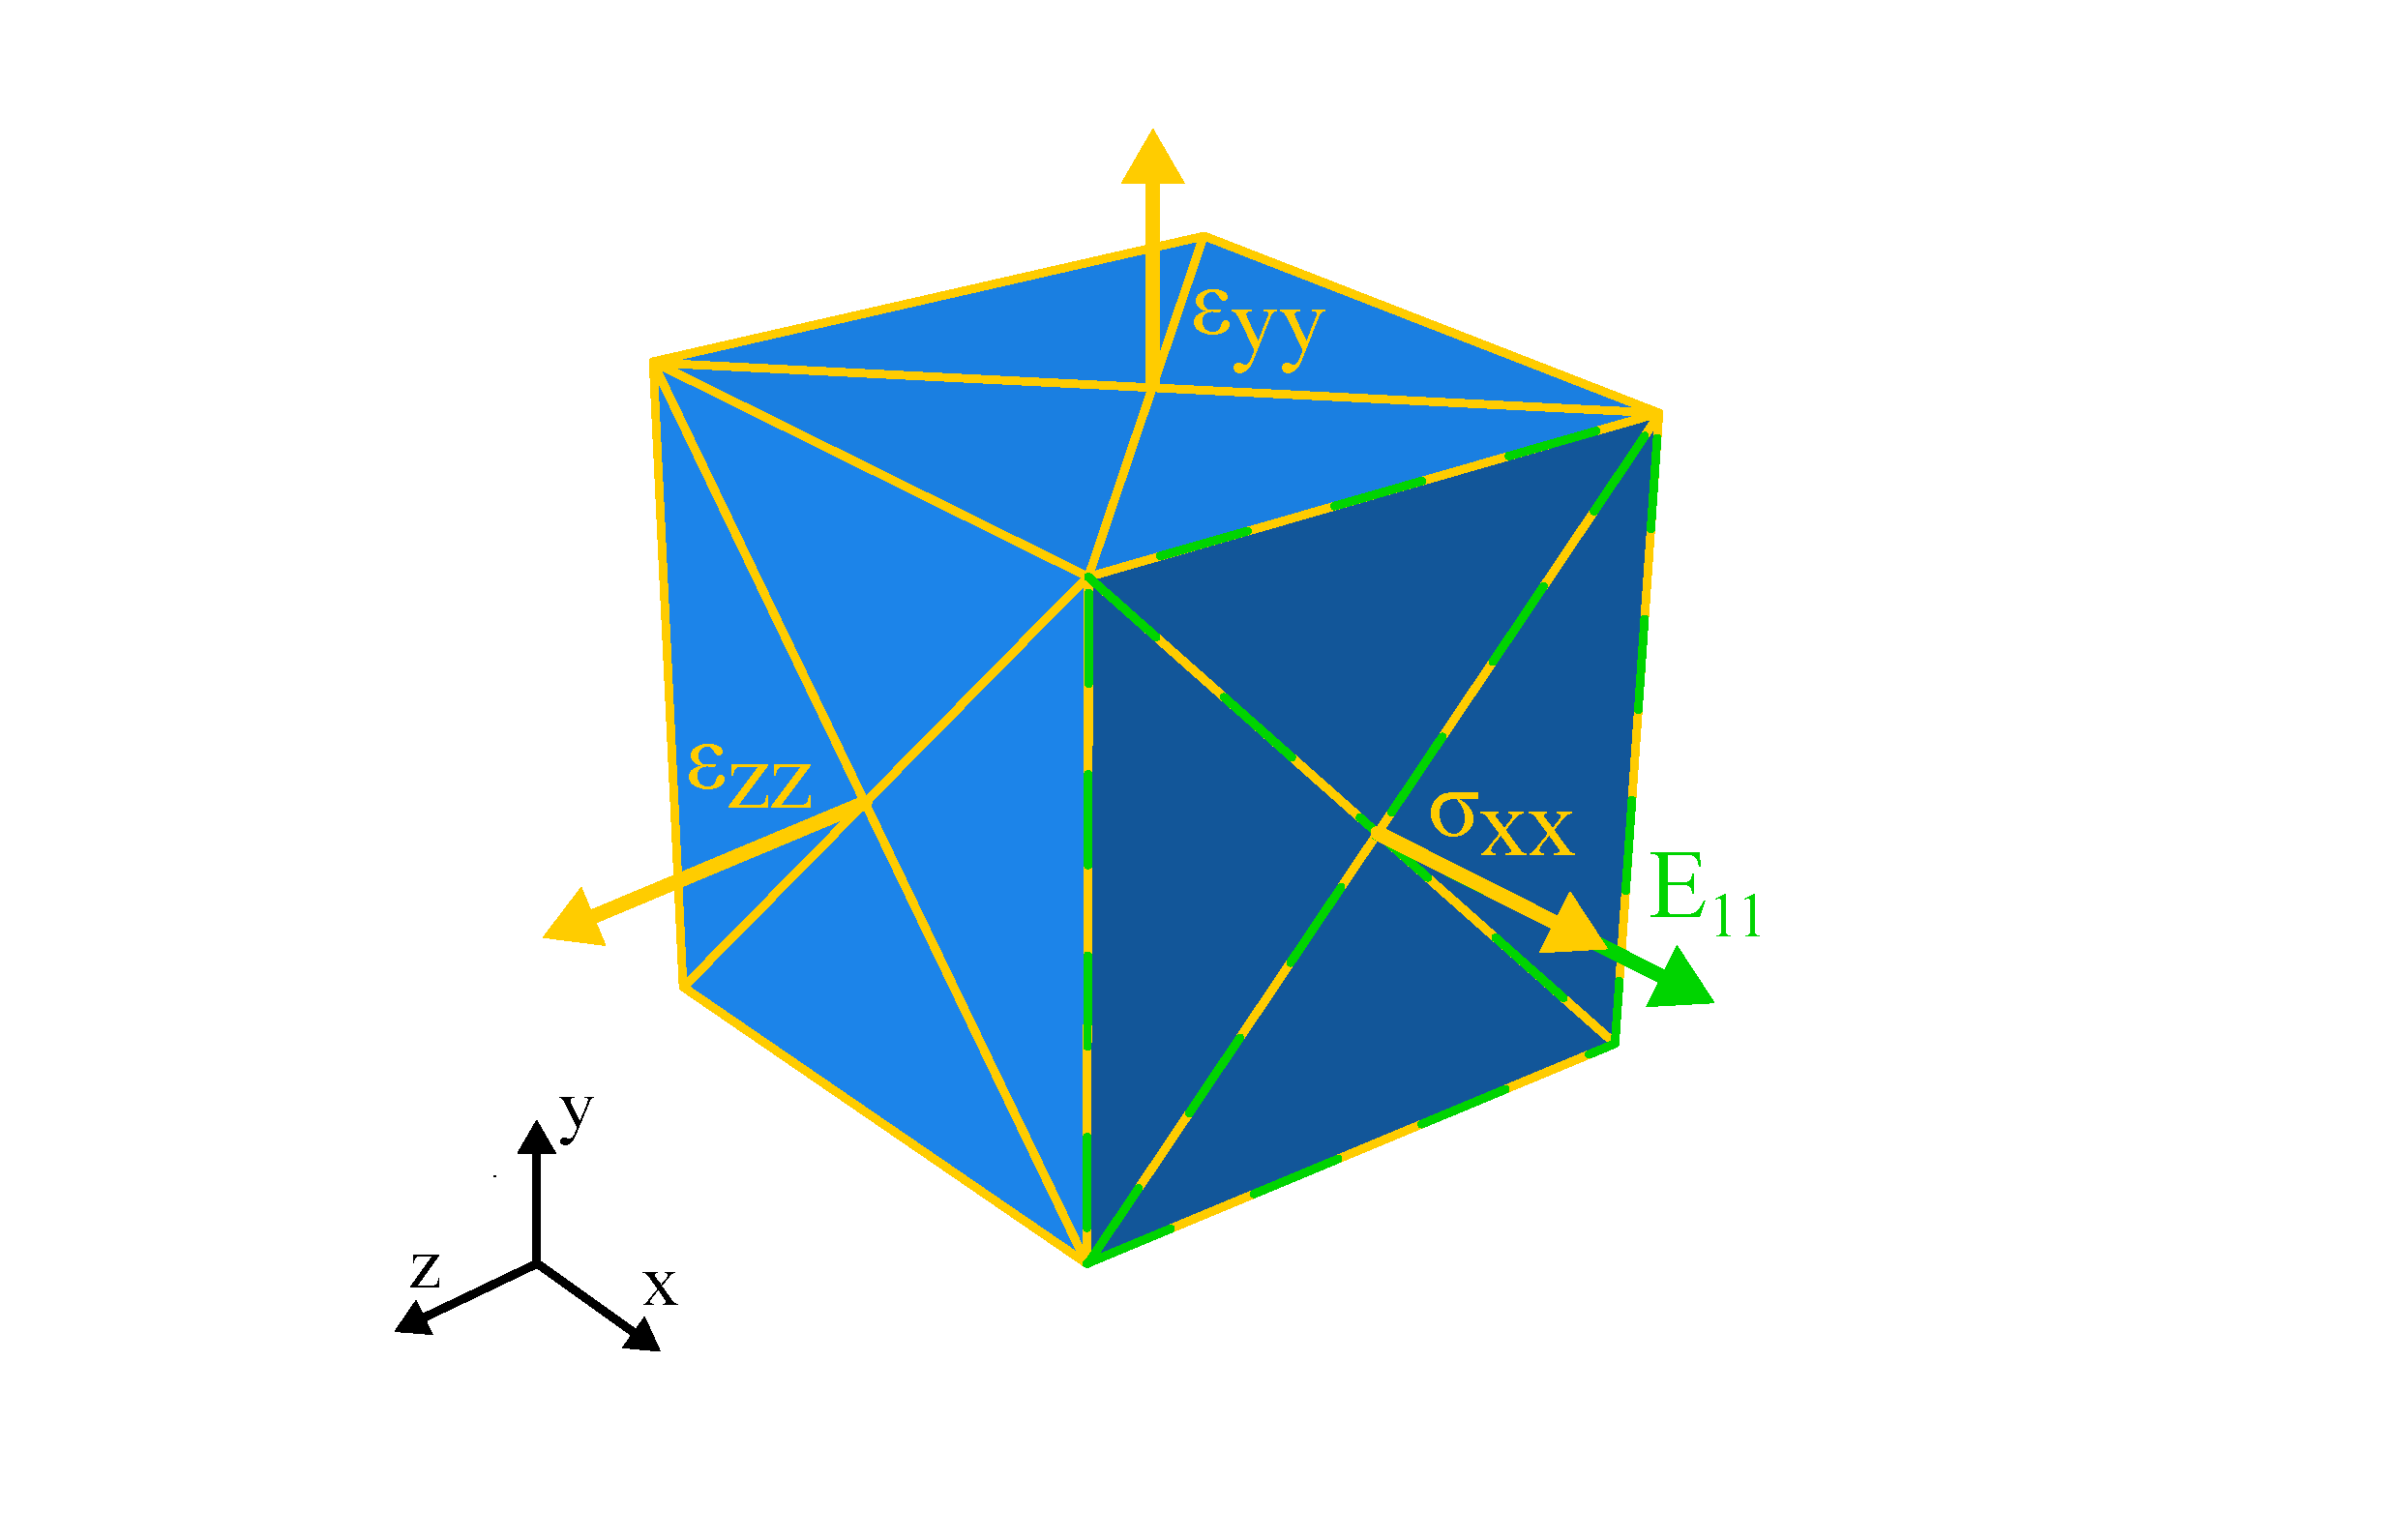
\includegraphics[width=0.7\textwidth]{cube_loading_plain_white_new.pdf}
		\caption{illustration of load case and evaluated stress and strain reactions}
		\label{fig:evaluationMeasurements}
	\end{figure}

    \subsection{Load parameters and load reactions}\label{subsec:loadParameters}
    In the optimisation process we use data from the MD-simulation as input-file. This input-file is called reference data. In contains stress and strain values in all normal and shear directions measured during the MD-simulation. They contain stress and strain values for multiple steps during the loading process. Thus, we can register different trends of loading and the corresponding responses.
    We split the reference data into load parameters and \acrfull{rlr}. The load parameters define the quantitative values of the prescribed load case. 
    Since we defined the load cases similar to the ones in the MD-simulations, we can use the data from the load parameters directly.  If we know the load case, we can easily extract the load parameters from the reference data and transfer them into the \name{abaqus} model. A detailed description of the load application in \name{abaqus} can be found in \autoref{sec: preprocessing}. 
    The \acrshort{rlr} represent the material response during the MD-simulation. From this, we extract the stress and strain values according to the chosen \acrlong{er} and neglect the other ones, since they probably contain little information about the material behaviour. Therefore we exclude this useless data from our definition of the \acrshort{rlr}.
    To perform the comparison of material behaviours we need analogous data from the \name{abaqus} simulation. From the odb we read out stress and strain values in all directions. Similar to the \acrshort{rlr} we extract the values corresponding to the \acrlong{er}. These values are called \acrfull{olr}. \\
    In \autoref{tab: testSeries} the load cases and load parameters we investigate in this work are shown.
    In the verification and validation studies we always apply a linear strain with a maximum value of 20\%. In the validation studies we use different mixing ratios as materials which show different mechanical behaviours. In the next study we investigate a tensile strain following a sinus function over time with a maximum amplitude of 15 \(\%\) strain. We only consider the first quarter of a period up to the maximum value as a preparation for studies with cyclic loading. In this preparing study we want to investigate the handling with non-linear loadings. Then we use the same load parameters but apply them as a shear strain. In the next step we use the same load parameters but combine the load cases of E11 and G12. Important to notice is that the previously introduced load parameters proceed in a wide strain range. Assuming that the material starts to plastify at XX, the majority of the loading steps are located in the plastic domain of the material. Conversely, the load parameters contain only little information about the elastic material behaviour. In \autoref{sec: verification} the issue about this unequal distribution in the material domains becomes clear.    
    As a last study we investigate  a full period of a sinusoidal loading for a tensile load case in x-direction. We use amplitudes of 1\(\%\), 5\(\%\) and 8\(\%\). Through the use of this load parameters we try to get a larger proportion of data points in the elastic domain.

    \begin{table}[H]
        \centering
        \renewcommand{\arraystretch}{1.3}
        \caption{Overview of test series, load cases and load parameters}
        \label{tab: testSeries}
        \begin{tabular}{L{0.17\textwidth}C{0.08\textwidth}C{0.13\textwidth}C{0.15\textwidth}C{0.13\textwidth}C{0.17\textwidth}}
        \toprule
        \multirow{2}{0.17\textwidth}{\textbf{Test series}} & \multirow{2}{0.08\textwidth}{\textbf{Load case}} & \multicolumn{2}{C{0.26\textwidth}}{\textbf{Load parameters}} &  \multirow{2}{0.13\textwidth}{\textbf{Mixing ratio}} &\multirow{2}{0.17\textwidth}{\textbf{Evaluated reaction}} \\ \cmidrule{3-4}
        & & \multirow{1}{0.13\textwidth}{\textbf{Trajectory}} & \multirow{1}{0.13\textwidth}{\textbf{Amplitude}} & & \\  \midrule
        Verification & E11 & Linear & 20\% & 6:3 & \(\sigma_{xx}, \varepsilon_{yy}, \varepsilon_{zz}\)\\\hline
        Validation I & E11 & Linear & 20\% & 4:3 & \(\sigma_{xx}, \varepsilon_{yy}, \varepsilon_{zz}\)\\ \hline
        Validation II& E11 & Linear & 20\% & 6:3 & \(\sigma_{xx}, \varepsilon_{yy}, \varepsilon_{zz}\)\\ \hline
        Validation III& E11 & Linear & 20\% & 8:3 & \(\sigma_{xx}, \varepsilon_{yy}, \varepsilon_{zz}\)\\ \hline
        \multirow{2}{0.15\textwidth}{Normal strain} & E11 & Sinus (\(\frac{1}{2} \pi\)) & 15\% & 6:3 & \(\sigma_{xx}, \varepsilon_{yy}, \varepsilon_{zz}\)\\ 
                &   &           &   && \\ \hline
        Shear strain  & E11 & Sinus (\(\frac{1}{2}\pi\)) & 15\% & 6:3 & \(\sigma_{xy}\)\\ \hline
        \multirow{2}{0.15\textwidth}{Normal \& Shear strain} & E11 & Sinus (\(\frac{1}{2}\pi\)) & 15\% & 6:3 & \(\sigma_{xx}, \varepsilon_{yy}, \varepsilon_{zz}, \sigma_{xy}\)\\ 
                                & G12 &       &      &     \\ \hline
        \multirow{2}{0.15\textwidth}{Normal strain} & E11 & Sinus (\(2\pi\)) & 1\%  & 6:3 & \(\sigma_{xx}, \varepsilon_{yy}, \varepsilon_{zz}\)\\ 
                    &     &       & 5\%  &  & \(\sigma_{xx}, \varepsilon_{yy}, \varepsilon_{zz}\)\\ 
                    &     &       & 8\%  & & \(\sigma_{xx}, \varepsilon_{yy}, \varepsilon_{zz}\)\\ \bottomrule
        \end{tabular}
        
    \end{table}



    \section{Error calculation}\label{sec: errorCalculation}
    As described in \autoref{sec: methodTheory} we have to compare the material behaviour in the \name{abaqus} simulation with the one during the MD-simulation. Therefore we use the reference load reactions and optimized load reactions. As described in \autoref{sec: methodTheory} the mathematical formulation of the optimisation problem requires the minimization of a scalar value. Since the load reactions consist of multiple values we need a method to condens the information from all load reaction values into a single value.  For a representative value we decide to build a \acrlong{rmse}. NOCH MEHR DAZU THEORIE. In the following we describe the procedure to compute this value.
    First we extract the \acrshort{rlr} and the \acrshort{olr}. In the next step we have to build the difference between them.  If we want to adequately describe the material behaviour it is sufficient to regard the load reactions during the complete loading process. Therefore we iterate over all load steps and compute the difference between the load reactions at the current load step. \autoref{fig: erroPlot} displays this procedure for an examplary set of \acrshort{rlr} and \acrshort{olr}. Here $\sigma_{xx}$ is the selected \acrlong{er}. For every load step $i$ their corresponding \acrshort{rlr} $\sigma_{i}^{\scriptscriptstyle RLR}$ and \acrshort{olr} $\sigma_{i}^{\scriptscriptstyle OLR}$ is logged. The blue arrow highlights their difference $\Delta\sigma_{i}$ for one examplary load step, according to \autoref{eq: EMDifference}. We square each of these differences to avoid negative values.  As described in \autoref{subsec:loadParameters} the distribution of the data points is unfavourable for the determination of the elastic parameters. To support the algorithm to find the elastic parameters anyway we applied a weight of 100 at the data point in the elastic domain. In the next step we build the mean value of the weighted arrays. The resulting value is called \acrfull{mse}. We compute the \acrshort{mse} for one \acrlong{er} according to \autoref{eq: mse}. Depending on the \acrlong{er} we compute $\text{mse}_{\sigma}$ or $\text{mse}_{\varepsilon}$. We have to compute this value for every selected \acrlong{er}. 

    \begin{center}
        \begin{gather}
            \label{eq: EMDifference}
            \Delta\sigma_{i} = \sigma_{i}^{\scriptscriptstyle RLR} - \sigma_{i}^{\scriptscriptstyle OLR} \hspace{2cm}
            \Delta\varepsilon_{i} = \varepsilon_{i}^{\scriptscriptstyle RLR} - \varepsilon_{i}^{\scriptscriptstyle OLR}\\
            \label{eq: mse}
            \text{mse}_{\sigma} = \frac{\displaystyle\sum_{i=1}^{N_{LS}} w_i (\Delta\sigma_{i})^2}{\displaystyle\sum_{i=1}^{N_{LS}}w_i } \hspace{2cm}
            \text{mse}_{\varepsilon} = \frac{\displaystyle\sum_{i=1}^{N_{LS}} w_i (\Delta\varepsilon_{i})^2}{\displaystyle\sum_{i=1}^{N_{LS}}w_i }
        \end{gather}
        \begin{equation*}
            N_{\text{LS}}: \text{Number of load steps}
            \hspace{1.5cm}
            w_i : \text{weight}
        \end{equation*}
    \end{center}
    
    
    
    For the tensile load case for example we have to do this for the \acrlong{er} $\sigma_{xx}, \varepsilon_{yy} \text{ and } \varepsilon_{zz}$. 
    If we now build one singular value out of these \acrshort{mse}s we have to ensure a common scale. Otherwise their influence on the overall error may vary significantly. Therefore it is necessary to apply weights to the mean squared errors of certain measurement quantities. The exact weights depend on the load case and the used load parameter set. In general, the \acrshort{mse} of \acrfull{eer} are much smaller than the ones from \acrfull{esr}, such that a weight of around 10e4 is necessary for the \acrshort{eer}. After that we sum up the weighted \acrshort{mse} and build again a mean value. From this value we build then the square root, as shown in \autoref{eq: rmse}. Since our code is able to process multiple load cases for one data set in one optimisation process we can calculate the \acrshort{rmse} for every load case and apply weights depending on the load case. Then we sum up all these weighted \acrshort{rmse} values. Additional, multiple load parameters sets can be processed which leads to a repetition of the described procedure for every load parameter set. Therefore we can calculate the return value for multiple load cases for multiple load parameter sets according to \autoref{eq: error}. Then we can apply weights for every load parameter set and sum it again to return a single value. This value is the one we return our minimization function. Through the adaption of the material values this value should be minimized. \\
    In the following sections we have a closer look on the implementation of this minimization process. 

    \begin{figure}[H]
        \centering
        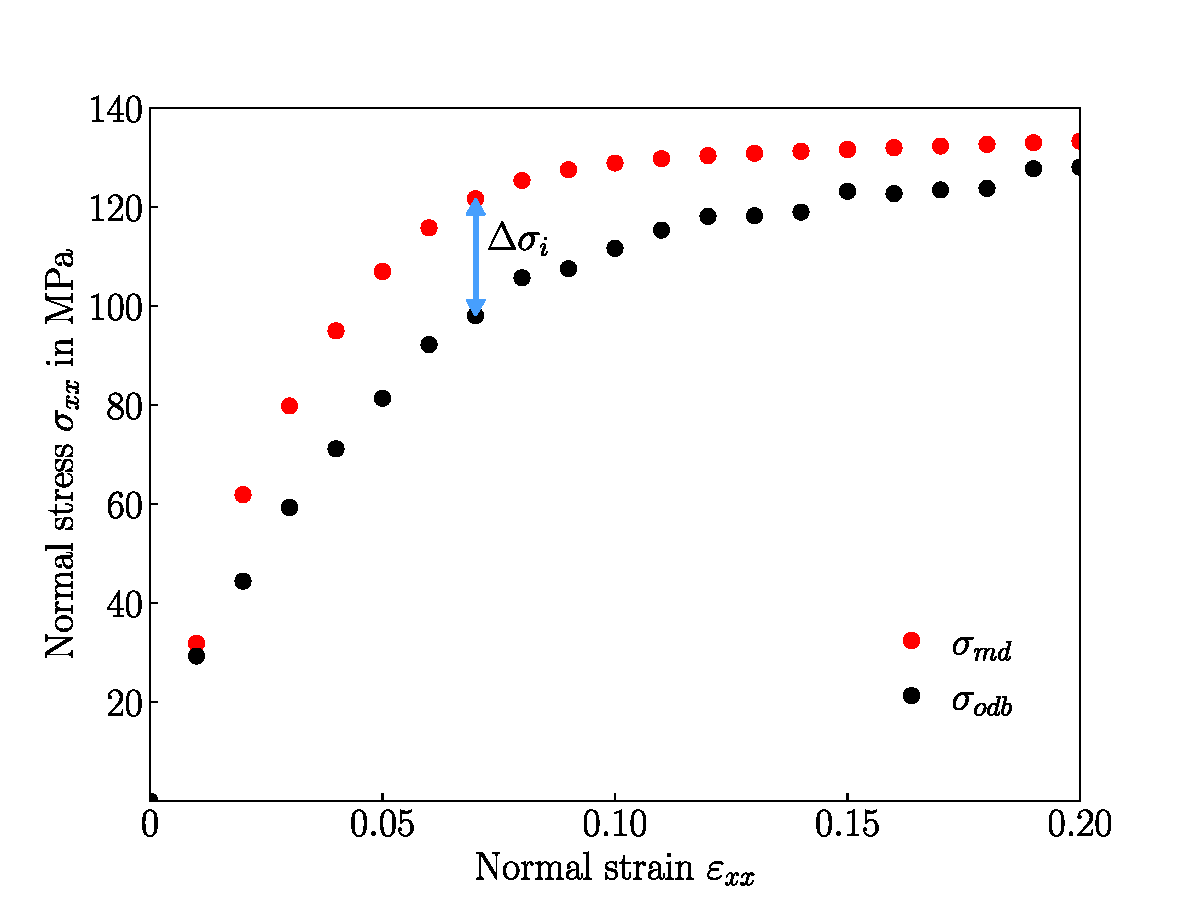
\includegraphics[width = 0.65\textwidth]{error_plot.pdf}
        \caption{Error plot}
        \label{fig: erroPlot}
    \end{figure}


    \begin{center}
        \begin{gather}
            \label{eq: rmse}
             \text{rmse} = \sqrt{\frac{\displaystyle\sum_{j=xx}^{N_\text{SED}} w_{\sigma} \cdot \text{mse}_{\sigma,j} + \displaystyle\sum_{j=xx}^{N_{EED}} w_{\varepsilon} \cdot \text{mse}_{\varepsilon,j}}{N_\text{SED} + N_{\scriptscriptstyle EED}}} \\
             \label{eq: error}
            \text{error} = \sum_{k=E11}^{N_\text{LC}} \sum_{l=1}^{N_\text{LP}} w_k w_l \cdot \text{rmse}_{k,l}  
        \end{gather}
        \begin{equation*}
            \begin{split}
                &N_\text{SED}: \text{Evaluated stress reactions}\\
                &N_{\text{LC}}: \text{Number of load cases}
            \end{split}
            \hspace{2cm}
            \begin{split}
                &N_\text{EED}: \text{Evaluated strain reactions}\\
                &N_{\text{LP}}: \text{Number of load parameter sets}
            \end{split}
        \end{equation*}
    \end{center}
    
 
    
    \section{Preprocessing} \label{sec: preprocessing}


    \begin{table}[H]
        \centering
        \caption{Input paramters for optimisation process}
        \renewcommand{\arraystretch}{1.1}
        \begin{tabular}{L{0.2\textwidth}C{0.2\textwidth}C{0.15\textwidth}C{0.1\textwidth}C{0.1\textwidth}}
        \toprule
        \textbf{Input parameter} & \textbf{Directions} & \textbf{Category} & \textbf{Data format} & \textbf{Unit} \\ \midrule
        Young's modulus & – & value    & array  & MPa \\ 
                    & – & minimum  & scalar & MPa \\ 
                    & – & maximum  & scalar & MPa \\ \hline
        Poisson's ratio  & – & value    & array  & –   \\ 
                    & – & minimum  & scalar & –   \\ 
                    & – & maximum  & scalar & –   \\ \hline
        Plastic Yield  & – & value    & array  & MPa \\ 
                    & – & minimum  & scalar & MPa \\ 
                    & – & maximum  & scalar & MPa \\ \hline
        \multirow{2}{0.2\textwidth}{Alpha, beta, gamma} & – & value    & array  & –   \\ 
                        & – & minimum  & scalar & –   \\ 
                        & – & maximum  & scalar & –   \\ \hline
        Load parameters & – & filename & string & –   \\ 
                        & – & weight   & scalar & –   \\ \hline
        Load case & \multirow{2}{0.2\textwidth}{E11, E22, E33, G12, G23, G13} & active & 0/1    & – \\ 
                &                               & weight & scalar & – \\ \hline
        Stress evaluation & \multirow{2}{0.15\textwidth}{xx, yy, zz, xy, yz, xz} & active & 0/1    & – \\ 
                        &                        & weight & scalar & – \\ \hline
        Strain evaluation & \multirow{2}{0.15\textwidth}{xx, yy, zz, xy, yz, xz} & active & 0/1    & – \\ 
                        &                        & weight & scalar & – \\ \hline
        Load weighting & \multirow{4}{0.2\textwidth}{normal stress, normal strain, shear stress, shear strain} & weight & scalar & – \\ 
        &&&& \\
        &&&& \\
        &&&& \\\bottomrule
        \end{tabular}
        
    \end{table}
    
    Before starting with the optimisation process, we need some preprocessing steps to prepare a working \name{abaqus} model with the required properties. In picture XX the complete structure of the code is depicted. The upper part belongs to the preprocessing. In the first step the code extracts the values from the input file. Table \autoref{tab:inputParameterTable} lists the input parameters relevant to the optimisation process. The whole input file is included in the Attachment XX. Here the user has multiple options to specify the optimisation process. It is possible to test multiple initial values for the material parameters calling the script once. This function is important to verify the optimisation results with varying input values. For every material parameter we can write an array of initial values. Then the code loops over all array entries at a time to extract one initial value for each parameter (see \autoref{tab:ModelSettings}). As a consequence all arrays need to be of same length. For all the created initial value combinations the code creates a new ModeldataBase (mdb) in \name{abaqus} and a new folder structure to set the working directory and store the results. \acrfull{mse}
    

    % \begin{table}[h]
    %     \begin{subtable}[c]{0.49\textwidth}
    %         \centering
    %         \renewcommand{\arraystretch}{1.1}
    %         \begin{tabular}{C{0.14\textwidth}|C{0.05\textwidth}C{0.05\textwidth}C{0.05\textwidth}C{0.05\textwidth}C{0.05\textwidth}}
    %         \toprule
    %             \multirow{2}{0.14\textwidth}{\textbf{Material parameter}} & \multicolumn{5}{C{0.25\textwidth}}{\textbf{Combinations}}\\
    %             & \textbf{1} & \textbf{2} & \textbf{3} & \textbf{4} & \textbf{5} \\ \midrule
    %             $E$     & $E_1$     & $E_2$      & $E_3$      & $E_4$      & $E_5$  \\
    %             $\nu$ & $\nu_1$ & $\nu_2$ & $\nu_3$ & $\nu_4$ & $\nu_5$ \\
    %             $\sigma_{pl}$ & $\sigma_{pl1}$ & $\sigma_{pl2}$ & $\sigma_{pl3}$ & $\sigma_{pl4}$ & $\sigma_{pl5}$ \\
    %             $\alpha$ & $\alpha_1$ & $\alpha_2$ & $\alpha_3$ & $\alpha_4$ & $\alpha_5$ \\
    %             $\beta$  & $\beta_1$ & $\beta_2$ & $\beta_3$ & $\beta_4$ & $\beta_5$ \\
    %             $\gamma$ & $\gamma_1$ & $\gamma_2$ & $\gamma_3$ & $\gamma_4$ & $\gamma_5$ \\
    %             \bottomrule
    %         \end{tabular}
    %     \end{subtable}
    %     \hfill
    %     \begin{subtable}[c]{0.49\textwidth}
    %         \centering
    %         \renewcommand{\arraystretch}{1.1}
    %         \begin{tabular}{C{0.14\textwidth}|C{0.05\textwidth}C{0.05\textwidth}C{0.05\textwidth}C{0.05\textwidth}C{0.05\textwidth}}
    %         \toprule
    %             \multirow{2}{0.14\textwidth}{\textbf{Material parameter}} & \multicolumn{5}{C{0.25\textwidth}}{\textbf{Combinations}}\\
    %             & \textbf{1} & \textbf{2} & \textbf{3} & \textbf{4} & \textbf{5} \\ \midrule
    %             $E$     & $E_1$     & $E_2$      & $E_3$      & $E_4$      & $E_5$  \\
    %             $\nu$ & $\nu_1$ & $\nu_2$ & $\nu_3$ & $\nu_4$ & $\nu_5$ \\
    %             $\sigma_{pl}$ & $\sigma_{pl1}$ & $\sigma_{pl2}$ & $\sigma_{pl3}$ & $\sigma_{pl4}$ & $\sigma_{pl5}$ \\
    %             $\alpha$ & $\alpha_1$ & $\alpha_2$ & $\alpha_3$ & $\alpha_4$ & $\alpha_5$ \\
    %             $\beta$  & $\beta_1$ & $\beta_2$ & $\beta_3$ & $\beta_4$ & $\beta_5$ \\
    %             $\gamma$ & $\gamma_1$ & $\gamma_2$ & $\gamma_3$ & $\gamma_4$ & $\gamma_5$ \\
    %             \bottomrule
    %         \end{tabular}
    %     \end{subtable}
    %     \caption{Parameterübersicht}
    % \end{table}


    

    \begin{table}[H]
        \centering
        \begin{minipage}[T!]{1.0\textwidth}
            \centering
            \begin{minipage}[T!][5.3cm][T!]{0.43\textwidth}
                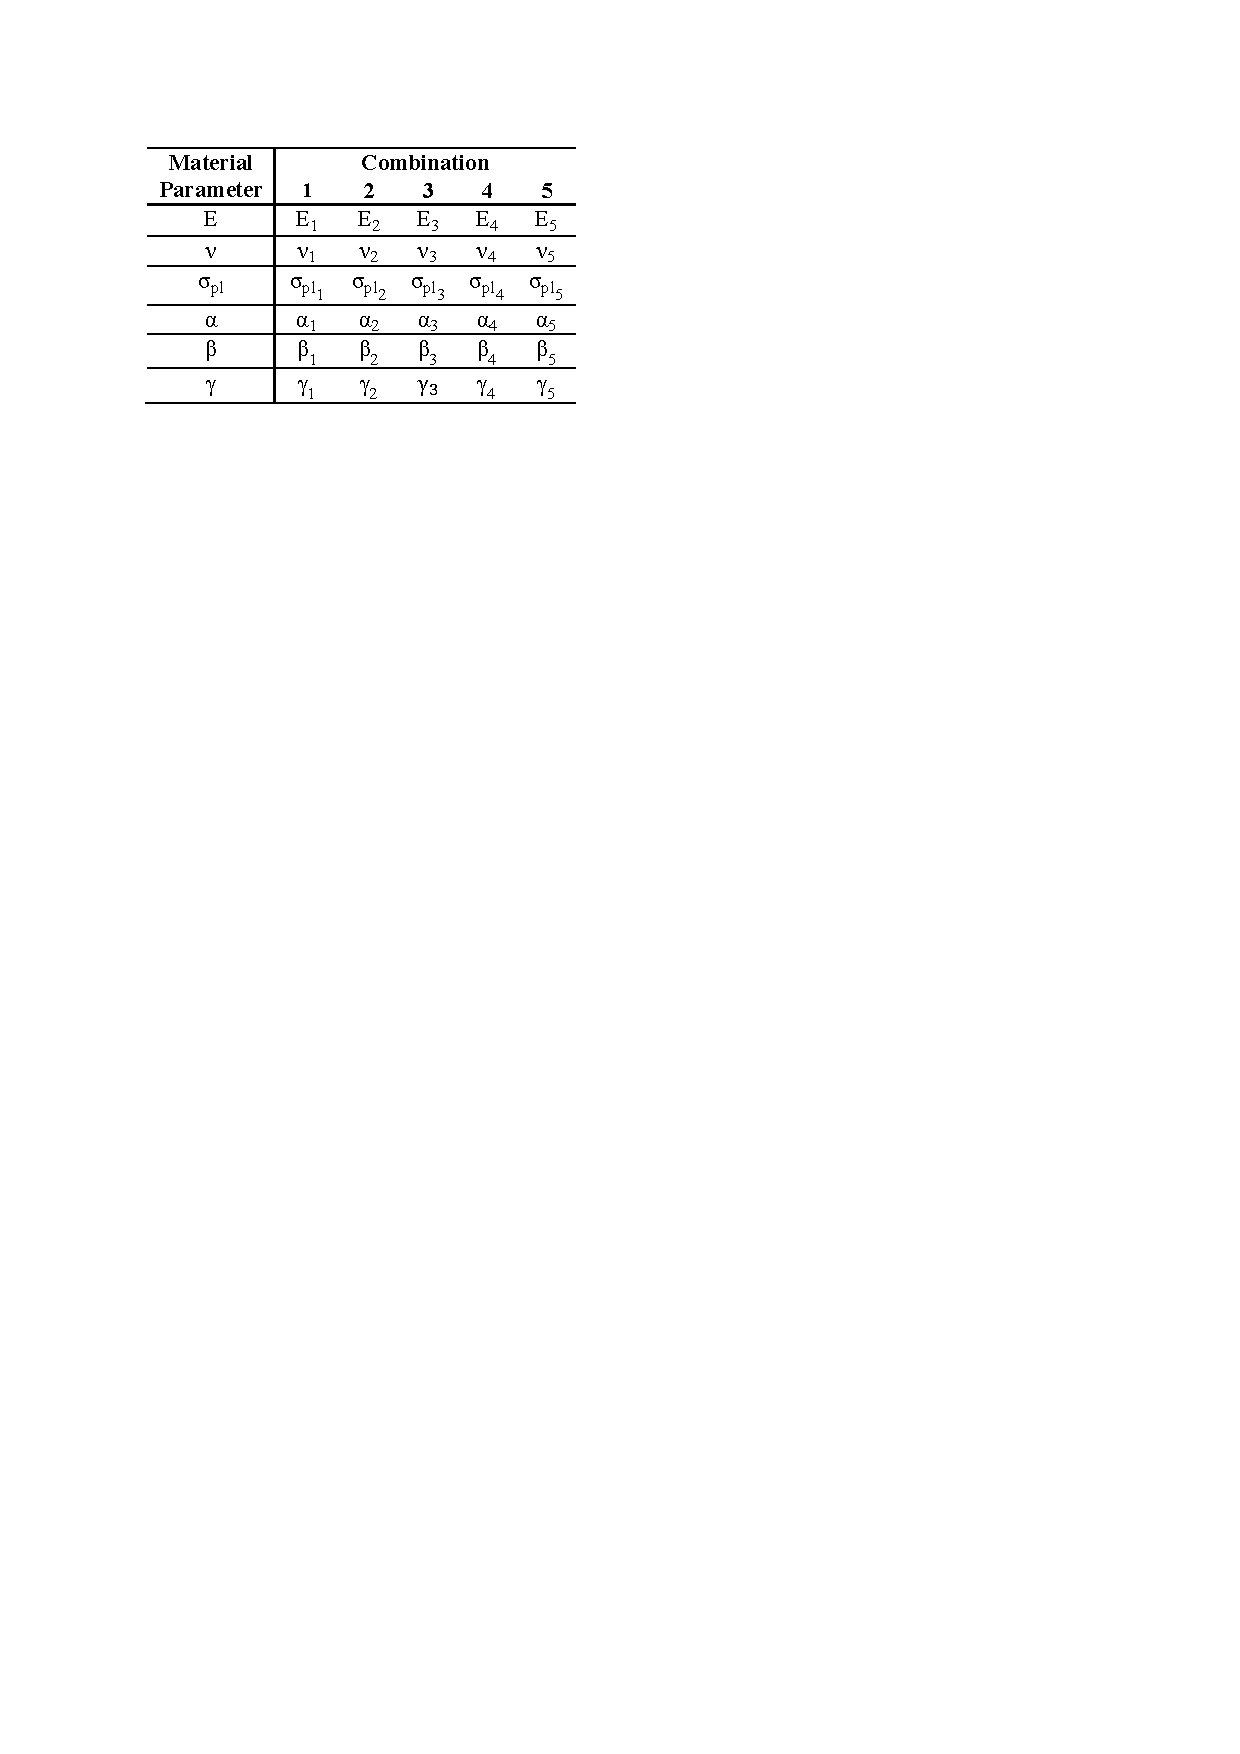
\includegraphics[width=1.0\textwidth]{initalValueComb.pdf}
                \vfill{}
		        \caption*{(a) Arrangement of initial value combination of material parameters}
                \label{tab:initialValueComb}
            \end{minipage}
            \hspace{0.05\textwidth} % Horizontal space between the minipage
            \begin{minipage}[T!][5.3cm][T!]{0.43\textwidth}
                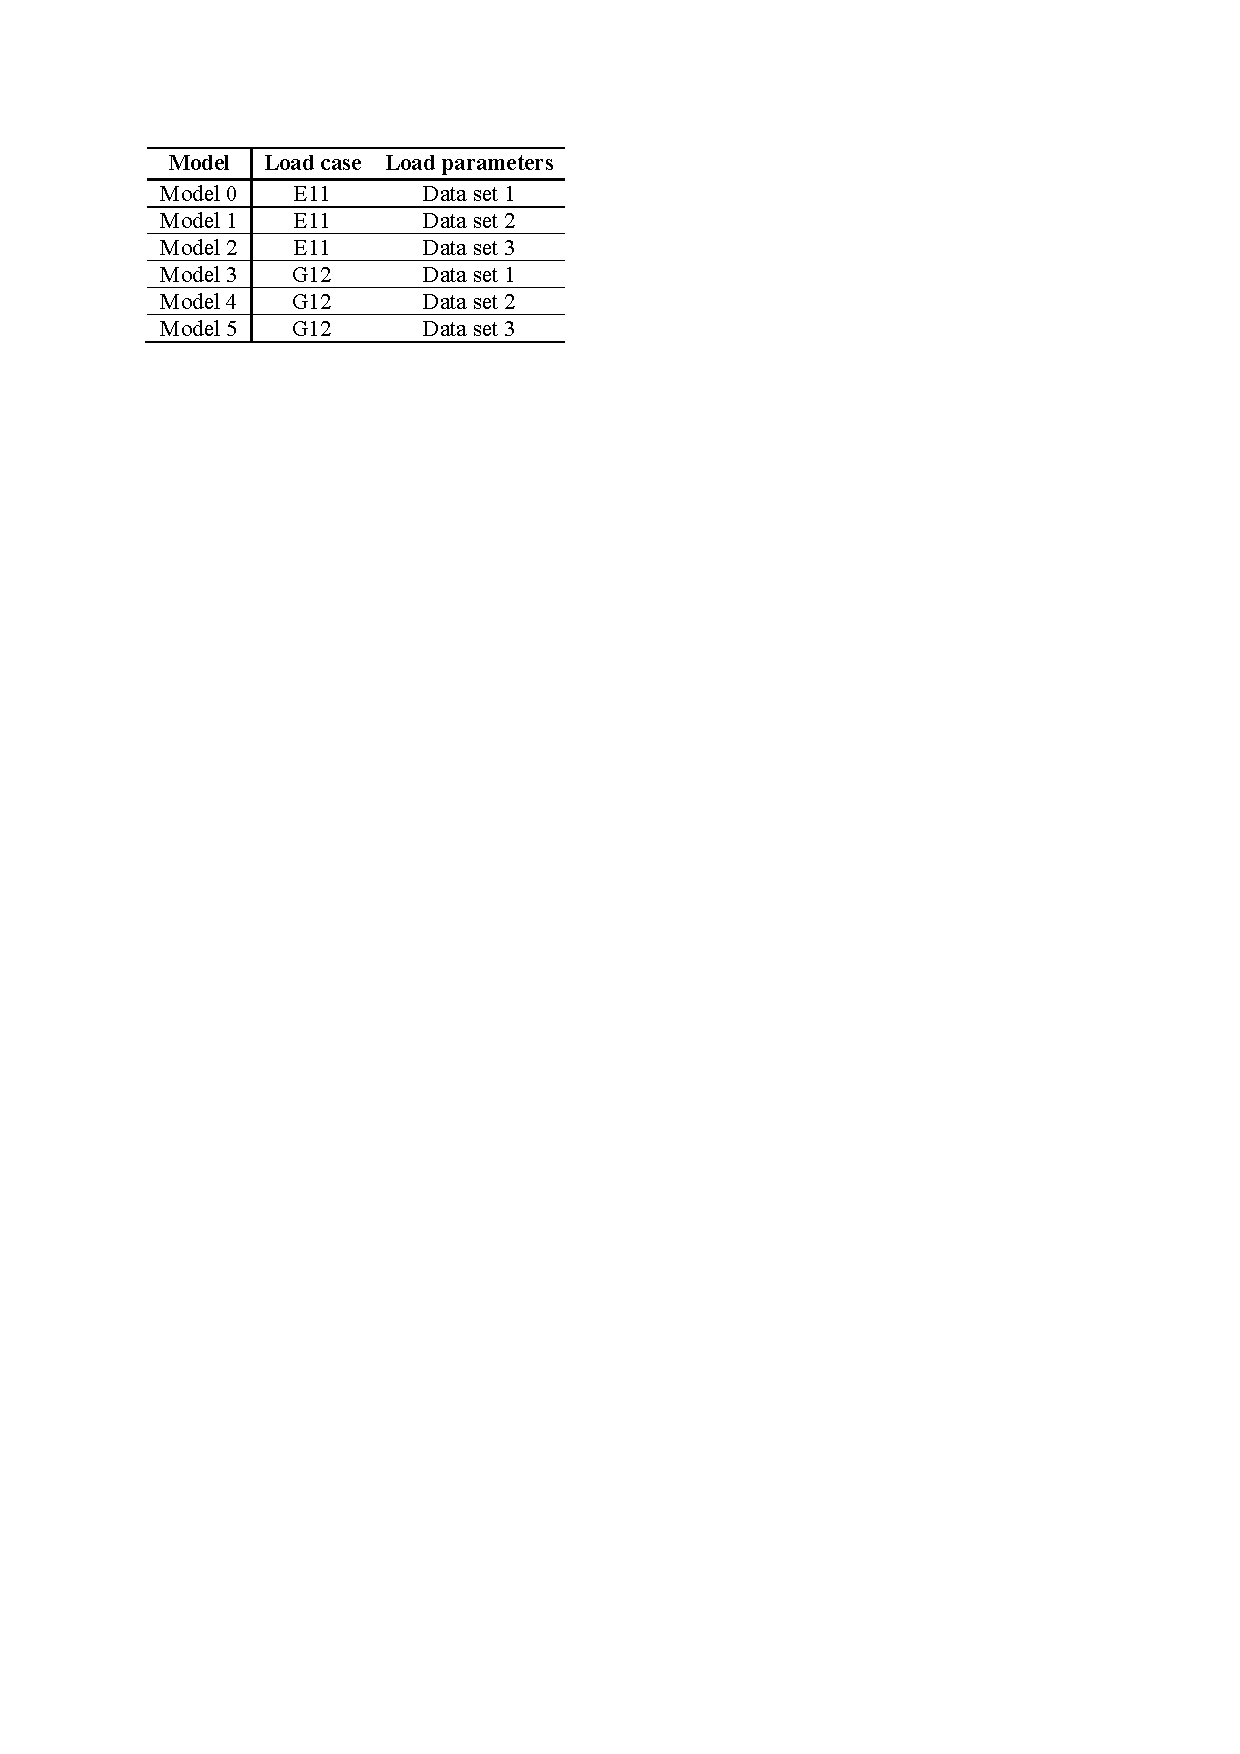
\includegraphics[width=1.0\textwidth]{ModelCombinations.pdf}
                \vfill{}
                \caption*{(b) Model creation for load case and parameter combinations}
                \label{tab:modelCombinations}
            \end{minipage}
        \end{minipage}    
        \caption{Loop conditions in preprocessing}
        \label{tab:ModelSettings}
	\end{table}
    
    Afterwards we start to construct the model. As discussed in section XX we use a cube with size 1x1x1 as model. We mesh the cube with 6x6x6 XXXX elements. The number of elements is a compromise between a coarse mesh for fast computation and a minimum number to avoid convergence errors. Although we use the hyperelastic material law in our optimisation process, we first have to build the model with elastic material. This is necessary for the usage of EasyPBC in the next step. Now we use the load case defined in the input file to create a EasyPBC job to apply it on the cube. As discussed in chapter XXX we use EasyPBC for the automatic construction of periodic boundary conditions. We use this set up to simulate a small detail of a infinitely large area (SCHLECHT FROMULIERT). Aside from that we use the generated boundary conditions for the applied load case. Since they act at a reference point a homogeneous load contribution is ensured. --> vlt auch in basics teil..
    However the settings from EasyPBC contain some default values, we have to adjust. EasyPBC applies for every load case a uniform displacement with a standard fixed value. In our optimisation we want to study cases with applied stresses as well. Additional we have to adapt the value of the load. For a correct comparison of the \name{abaqus} data with the MD-data we have to create evaluation points at similar load increments. In \name{abaqus} we can solve this issue by creating an amplitude. We register the evaluation points from the MD-data as steps and use this amplitude to apply the load. The value of the load is then set to 1 because it only defines the factor the amplitude is multiplied (see \autoref{fig:ABAQUS Settings}). Afterwards we modify the increment settings. EasyPBC automatically creates increments with fixed size and without non-linear geometry effects. In order not to run into convergence errors we use automatic incrementation. Especially in the first load steps we observe large deformations. If we try to resolve such large deformations in one incrementation step \name{abaqus} cannot resolve the step. With automatic incrementation \name{abaqus} can adapt the number of increments per load step dynamically. The non-linear geometry effects have to be considered because of the material properties we use. As described before we build elastic material for the usage of EasyPBC. In the following the code removes this material and substitutes it with a hyper-elastic material which is suitable for high non-linear deformation. By using this material, \name{abaqus} demands the inclusion of non-linear geometry effects. In the last step of preprocessing we store the model in a dictionary. We use this dictionary later to call the models for the optimisation. We perform the preprocessing for all prescribed load cases. This means for example if we define E11, G12, and G23 as load cases, we create one model for each load case in the previous described manner. Furthermore, we loop over the load parameters and create separate models. In the end we have then for each combination of load case and load parameter one model. 

 

     \begin{figure}[H]
        \centering
        \begin{minipage}[T!]{1.0\textwidth}
            \centering
            \begin{minipage}[T!][9cm][T!]{0.35\textwidth}
                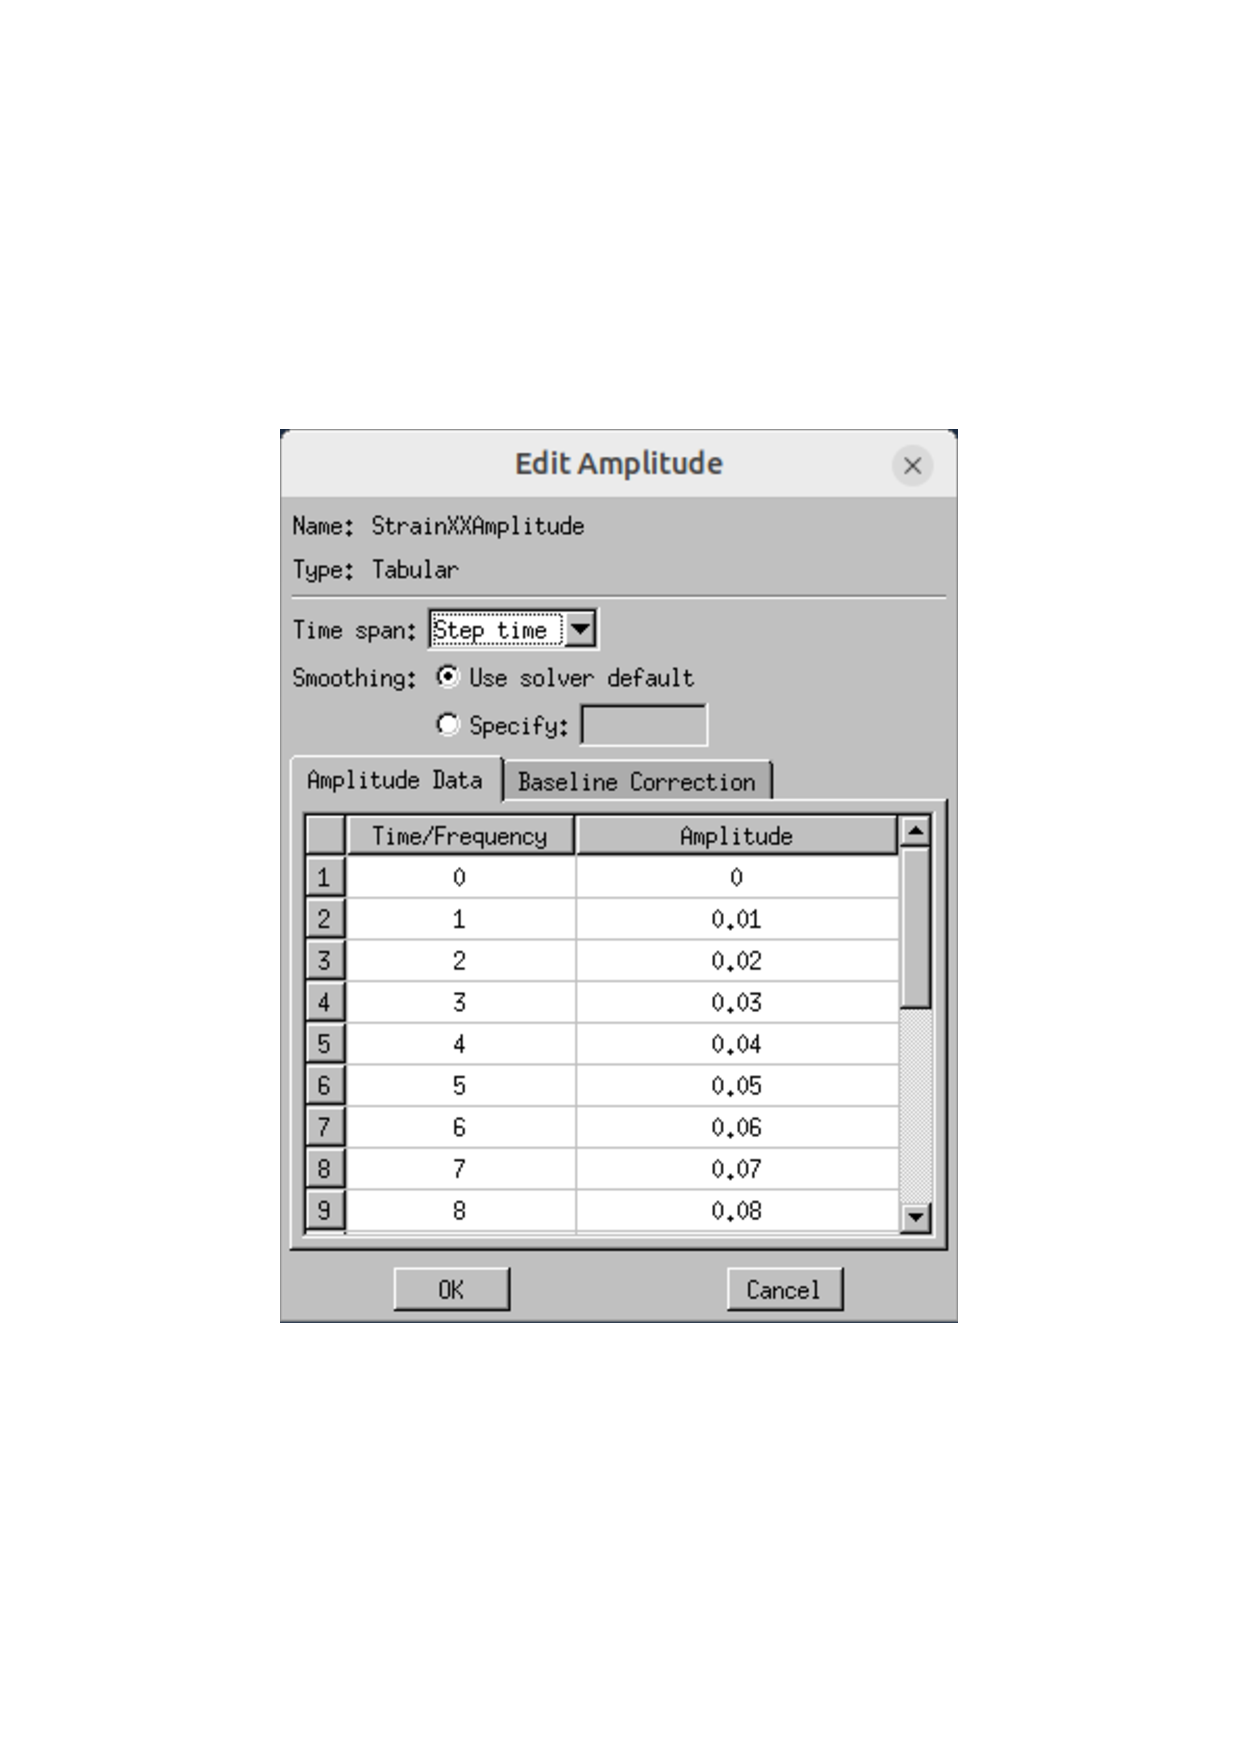
\includegraphics[width=1.0\textwidth]{Amplitude.pdf}
                \vfill{}
                \caption{Definition of load amplitude in \name{abaqus}}
                \label{fig:amplitudemenu}
            \end{minipage}
            \hspace{0.08\textwidth} % Horizontal space between the minipage
            \begin{minipage}[T!][9cm][T!]{0.35\textwidth}
                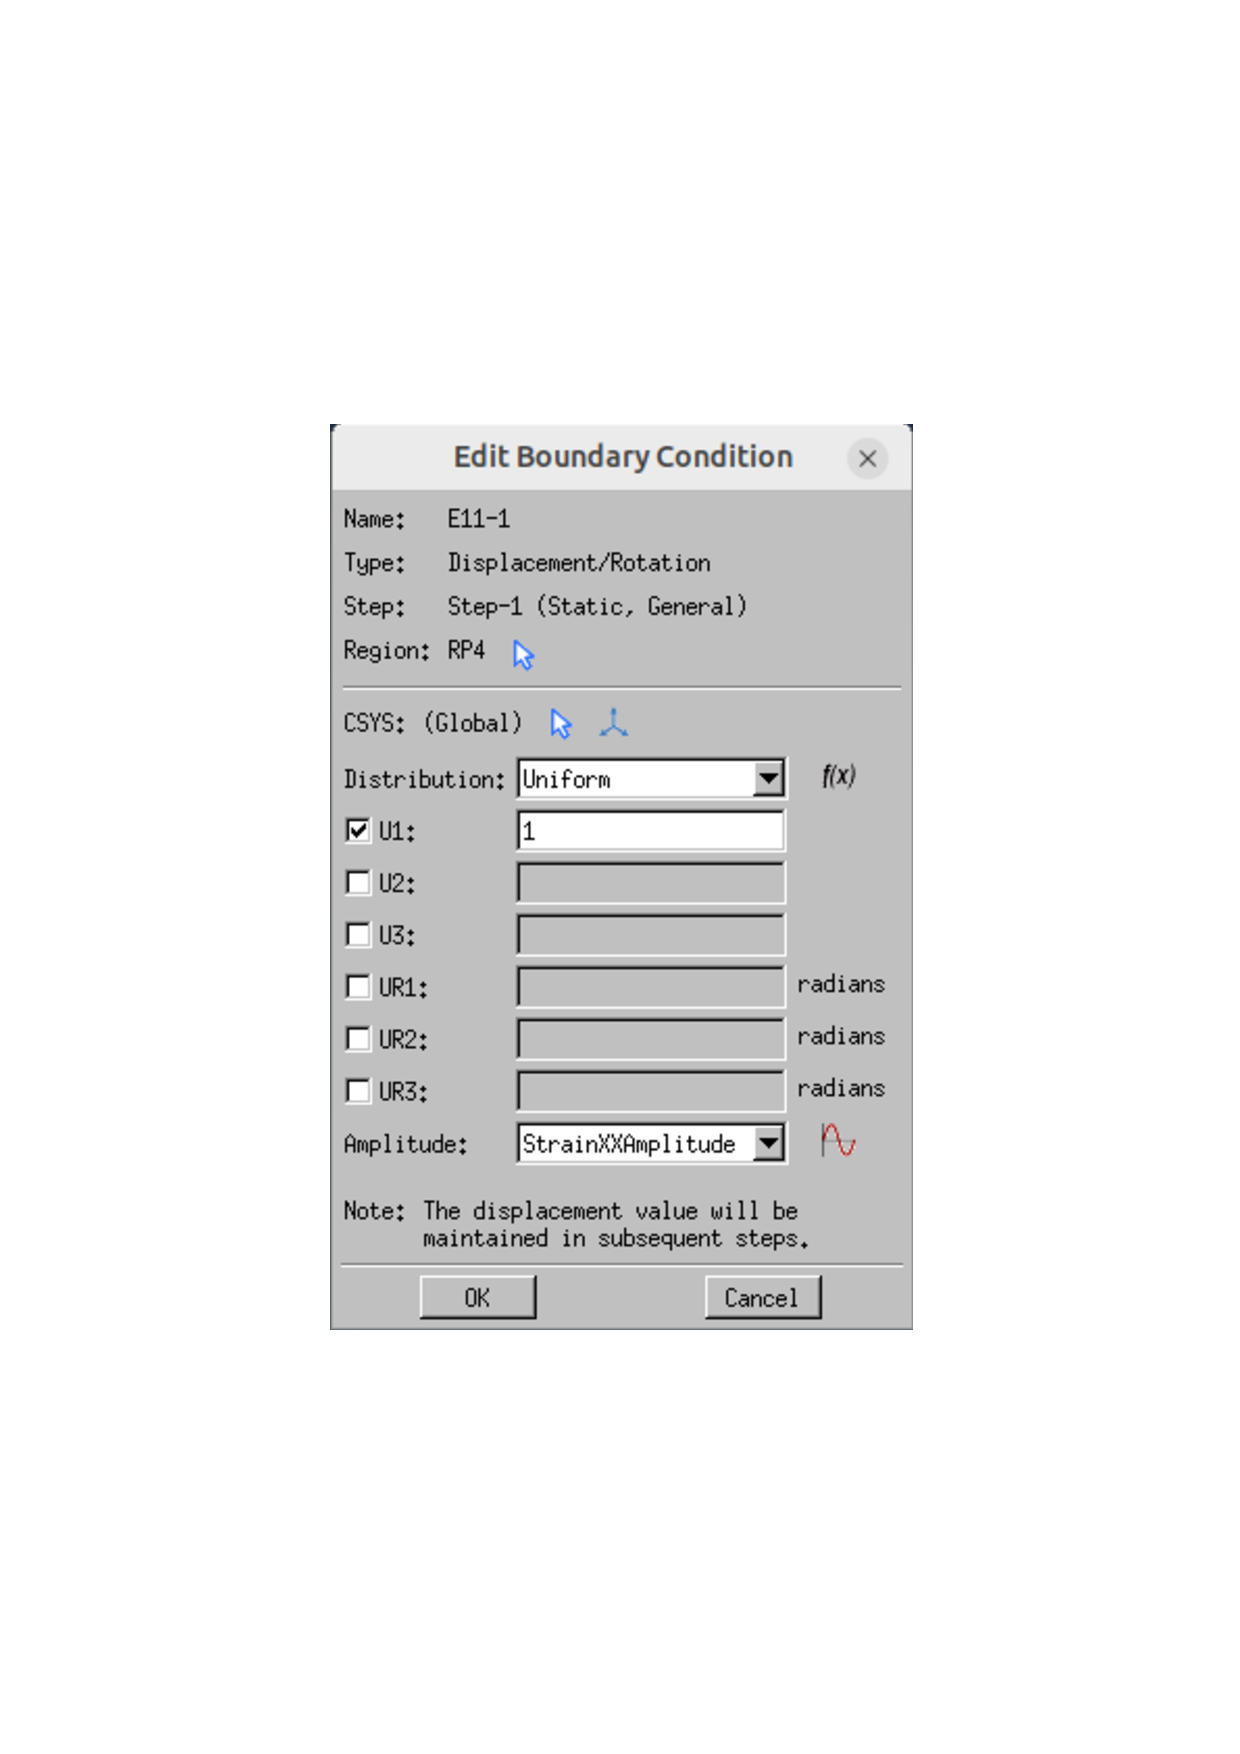
\includegraphics[width=1.0\textwidth]{BC.pdf}
                \vfill{}
                \caption{Boundary condition menu in \name{abaqus}}
                \label{fig:bcmenu}
            \end{minipage}
        \end{minipage}    
        \caption{Loop conditions in preprocessing}
        \label{fig:ABAQUS Settings}
	\end{figure}
 
    \section{Optimization process} \label{sce: optimizationCode}

     \begin{table}[H]
		\centering
        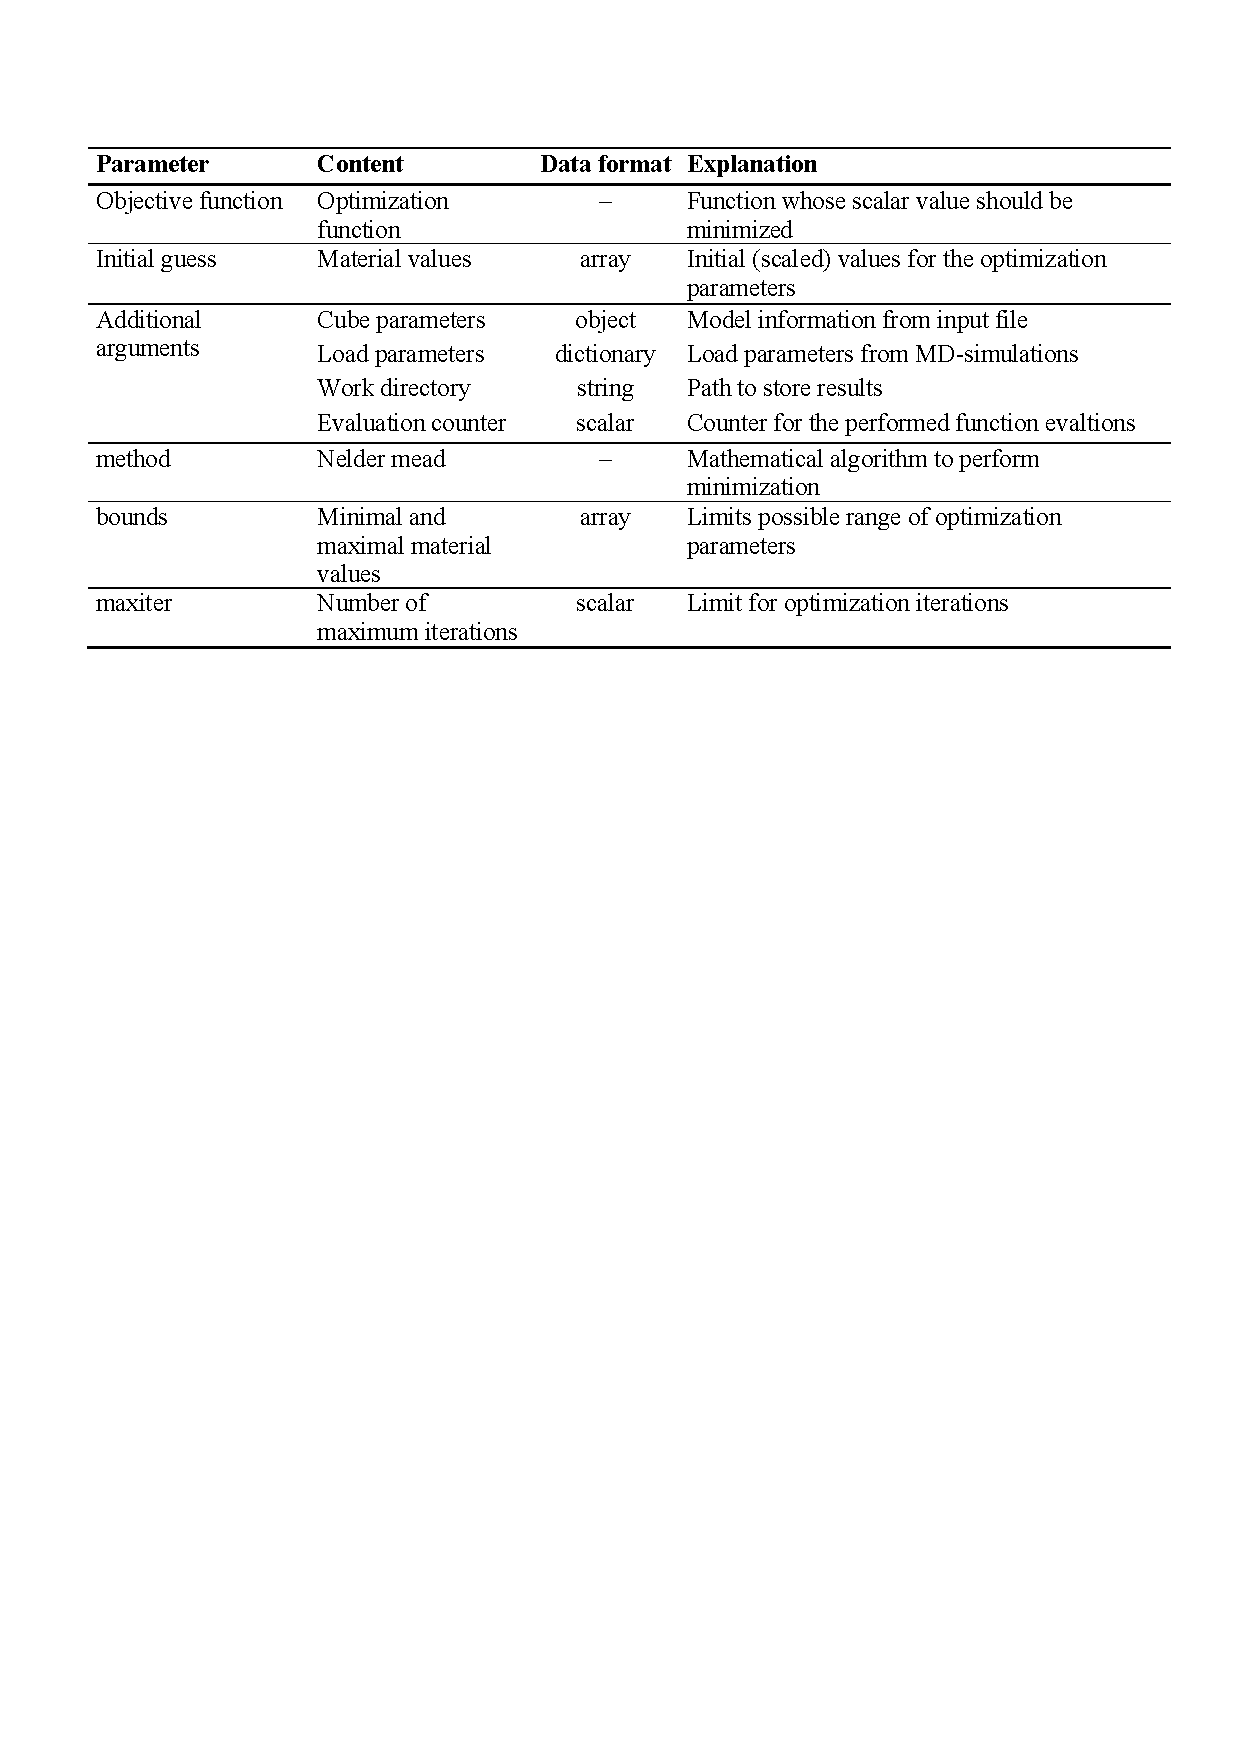
\includegraphics[width=0.95\textwidth]{minimizeFuncitonInput.pdf}
		\caption{Input parameters for SciPy minimize function}
		\label{tab:minimizeFunctionInput}
	\end{table}

    In the following section we describe the optimisation process. We start the processing by calling the scipy-minimize function. We pass this function various parameters to perform the optimisation listed in table XX. (MEHR ÜBER INPUT PARAMETER INKL TABLEE ) The minimize function itself calls our self-written optimisation function, where the evaluation takes place. As described before we create a model with a corresponding job for every combination of load case and load parameters and store them in a dictionary. Now we pass the whole dictionary to the optimisation function. All of the models describe now different test cases for the same material. We want to use them all to get as much information as possible, such that we have to include all of them into the optimisation process. To do so we have to calculate an error expression from all these analyses as described in section XX. 
    We start the process with rewriting the material values in all models. Since they all describe the same material we write the same values for every model. For the minimization computation optimisation parameters are scaled in the bounds 0-1, that we have to rescale them first. Then we can use the rescaled parameters to compute the values for the plastic stress function with the formula for VOCE-hardening. Now we can update all material values. in the next step we handle the models successively. We start a job to perform the \name{abaqus} analysis and open the resulting output-data base. Afterwards we read the stresses from the odb. We do this by reading the fieldOutput variable 'S' and write the data in a stress directory. Since we need the stress-values at all the defined strain steps we read out every frame. One frame corresponds with one strain step. Additionally we loop over all directions (xx, yy, zz, xy, yz, xz). The same procedure is done for the strain values. Here it is important to read out the correct strain variable 'NE' (nominal strain). For hyperelastic materials \name{abaqus} uses as standard value the logarithmic strain ('LE'), which gives incorrect values in our studies. Then we store all values for all frames and directions in a dictionary again. Now we collected all required data to calculate the error. We do this in the way described in section XX. For a better structure of the code this part is outsourced in a separate function. We call this function and pass the stress and strain directory as well as the corresponding load parameters from the md-analysis. Then the computation runs and the function returns the rmse value for this job. Multiplied with its corresponding weights for load case and load parameters we add this value to the total error value. Now we restart the result reading and error computation for the next job. When all jobs are processed we have a total error value containing information from all jobs about the quality of the current material values. This value is the one we return our minimization function. It uses this values to compute internal the next material value combination to reduce the returned error value. Now one optimisation iteration is performed. The new combination of material values is passed to our optimisation function and it starts again. This process will run till our defined number of maximum iterations is reached. 

    % \begin{enumerate}
    %     \item call scipy minimize with all necessary arguments
    %         1. function which shuold be minimized
    %         2. list with optimisation parameters
    %         3. additional arguments: data which are called in the minimized function:
    %             cubeparameter- object, mddaa dictionary, work directory, evaluation counter
    %         4. minimization method: nelder mead
    %         5. boundaries for optimisation parameters
    %         6. options: return all (return function value from every iteration), maxiter (use max iteeration value as termination criterion)
    % \end{enumerate}

    % optimisation function:
    % \begin{enumerate}
    %     \item rescale material parameters
    %     \item compute plastic stresses
    %     \item delete elastic material
    %     \item write hyperelasitc material and update plastic material
    %     \item delete lock-files for job: they prevent the start of a job where a obd is already written
    %     \item list jobs in current work directory/ mdb
    %     \item iterate over jobs
    %     \item start job
    %     \item open odb
    %     \item create stress directory: for tensile load cases with normal direction, for shear load with shear direction
    %     \item loop over all directions
    %     \item loop over all frames from last step
    %     \item read fieldoutput 'S' from element set in current direction 
    %     \item write it in stress directory
    %     \item create strain directory
    %     \item loop over all directions
    %     \item loop over all frames from last step
    %     \item read fieldoutput 'NE' from element set in current direction 
    %     \item write it in strain directory
    %     \item call calculate rmse function
    %     \item call multiple save functions to store results
    %     \item when all jobs are finished: 
    %     \item multiple rmse from jobs with weights from parameter input (different weighting of load cases or md data sets)
    %     \item sum weighted rmse 
    %     \item save material parameters, rmse
    %     \item return total rmse

    % \end{enumerate}

    
    
    % calculate rmse function:

    % \begin{itemize}
    %     \item loop over directions in stress directory if the direction should be anaylsed (parameter input)
    %     \item read out md data for this direction
    %     \item check if md data and odb data have the same length
    %     \item calculate squared differences for every step (array)
    %     \item weight array --> first data point is weighted with 100, because it is the only point in elastic domain 
    %     \item compute mean from array: sum over all weighted squared differences/ sum of all weights
    %     \item differentiate between tensile and shear load case:
    %         - use correlated weight 
    %     \item append to mse array
    %     \item same procedure  for strain directory
    %     \item sum up all mse values, divide by number of values (build mean value)
    %     \item wurzel ziehen
    %     \item return rmse
    % \end{itemize}
        
    
    
    
    % - formel wir sich RMSE zusamensetzt
    % - welche schleifen gibt es?
    

    % test cases:
    % - linearere Zug
    % - Zug und shear --> mit sinusform --> warum? 
    % - cyclic tensile 
    